\chapter{Fejlesztői dokumentáció} % Developer guide
\label{ch:impl}

\section{Tervezés}

\subsection{Feladat leírása}

Az alkalmazás két részből áll, egy böngészős frontendből és egy szerveren futó backendből. Az alkalmazás funkcióit a \ref{sec:functionDefinitions} részben írtam le bővebben. Tervezés szempontjából a funkcionális követelmények a következők:

\begin{compactitem}
	\item Egy kategória látható egy felhasználónak, ha: nyílt a kategória, a felhasználó hozta létre a kategóriát, a felhasználó engedélyezve van a kategórián, a felhasználó résztvevő egy időponton ami aminek ez a kategóriája
	\item Egy időpont látható egy felhasználónak, ha látható a kategóriája vagy ha résztvevő az időponton
	\item Kategóriát nem lehet törölni
	\item Profilkép feltöltésnél validálni kell a fájl típusát és méretét
	\item Ha a felhasználó böngészőjében van bejelentkezési süti, akkor automatikusan jelentkeztesse be a weboldal
\end{compactitem}

Az alkalmazás nem funkcionális követelményei a következők:

\begin{compactitem}
	\item Intuitív, egyszerűen használható felhasználói felület
	\item Egyszerre több felhasználó is használhatja az alkalmazást, egyszerűen skálázható legyen a rendszer.
	\item A felhasználói interakciók (pl.: új időpont hirdetés, időpont foglalás) ne frissítse az ablakot, történjen meg egyből, reaktívan.
\end{compactitem}

\clearpage

\subsection{Felhasználói esetek}
A felhasználói esetek a következőképpen néznek ki. A vállalkozó egyben ügyfél is (hogy esetleg más vállalkozók időpontjaira tudjon jelentkezni), az ügyfelek összes funkcióját tudják használni, ezt nem jelöltem a diagrammban, hogy átlátható maradjon.

\begin{figure}[H]
	\centering
	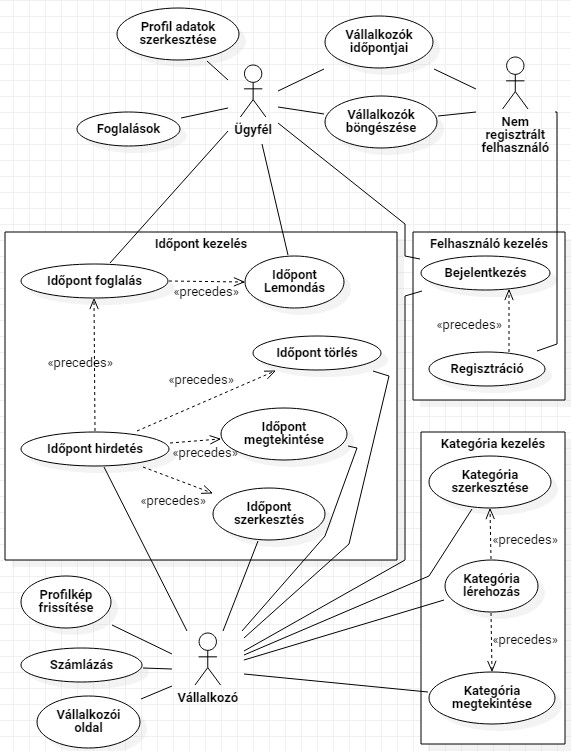
\includegraphics[width=0.9\textwidth]{usecase3}
	\caption{Felhasználói esetek}
	\label{fig:usecases}
\end{figure}


\todo{given when then}

\begin{table}[H]
	\centering
	\begin{tabular}{|l|l|c|}
		\hline
		& \textbf{Leírás} & \textbf{Kód} \\
		\hline
		GIVEN & Nincs bejelentkezve & \multirow{3}{*}{asd} \\ \cline{1-2}
		WHEN & Bejelentkezéshez kötött oldalt nyitna meg & \\ \cline{1-2}
		THEN & Visszairányítódik a főoldalra & \\ 
		\hline
		GIVEN & asd & \multirow{3}{*}{asd} \\ \cline{1-2}
		WHEN & asd & \\ \cline{1-2}
		THEN & asd & \\ 
		\hline
		GIVEN & asd & \multirow{3}{*}{asd} \\ \cline{1-2}
		WHEN & asd & \\ \cline{1-2}
		THEN & asd & \\ 
		\hline
		GIVEN & asd & \multirow{3}{*}{asd} \\ \cline{1-2}
		WHEN & asd & \\ \cline{1-2}
		THEN & asd & \\ 
		\hline
		GIVEN & asd & \multirow{3}{*}{asd} \\ \cline{1-2}
		WHEN & asd & \\ \cline{1-2}
		THEN & asd & \\ 
		\hline
		GIVEN & asd & \multirow{3}{*}{asd} \\ \cline{1-2}
		WHEN & asd & \\ \cline{1-2}
		THEN & asd & \\ 
		\hline
		GIVEN & asd & \multirow{3}{*}{asd} \\ \cline{1-2}
		WHEN & asd & \\ \cline{1-2}
		THEN & asd & \\ 
		\hline
	\end{tabular}
\end{table}

\subsection{REST API vs MVC architektúra}
Webes alkalmazások körében régebben elterjedt volt a Modell-View-Controller architektúra (röviden MVC). Röviden ez azt jelenti, hogy a felhasználó akcióira a Controller réteg eldönti, hogy az állapotot (Modellt) hogy kell frissíteni, ez után pedig egy nézetet (View-t) ad vissza a felhasználónak. A gyakorlatban ez szerver oldali renderelést jelent, például a felhasználó elküld egy űrlapot a szervernek, az feldolgozza és egy szerver által renderelt HTML fájlt küld vissza a felhasználó böngészőjének.

Ennek a megközelítésnek vannak előnyei, többek között, hogy az alkalmazásnak egy kódbázisa van, egyszerűbb egy új funkciót implementálni, kevesebb technológiát is elég ismerni. Hátránya viszont, hogy dinamikus felhasználói felületet nehéz benne építeni, más alkalmazásokba, például mobil alkalmazásba, nem lehet integrálni.

Ezekre nyújt megoldást, ha a logikát egy REST API\footnote{Representational state transfer, Application Programming Interface} valósítja meg backenden, a megjelenítésért pedig egy másik program felel frontend-en. A REST egy interfész leíró struktúra, legtöbb esetben HTTP protokoll alapú kommunikációt ír le, melyben JSON\footnote{JavaScript Object Notation} formátumú adattal lehet kommunikálni.

Mivel az API-t így programatikusan tudjuk elérni, ezért más alkalmazásokkal egyszerűen képes kommunikálni. Így lehet például web-ről, telefonos- vagy asztali alkalmazásból elérni ugyan azt a biznisz logikát, ezért csak a megjelenítést kell variálni platformok között.

A REST API állapot mentes, ami azt jelenti, hogy a szerver nem függ valamilyen kontextustól, csak a kérésben szereplő adattal elég dolgoznia. Ez lehetővé teszi, hogy a backend több szerveren horizontálisan egy load balancer (terheléselosztó) segítségével legyen skálázva. Egy ilyen rendszerben az egymást követő kérések akár különböző backend példányokhoz futhatnak be, az alkalmazás ugyan olyan pontosan működik.

A programozható felület lehetővé teszi, hogy a szerver ne teljes oldalakat küldjön vissza válasznak, hanem csak adatot. Ez a rugalmasság lehetővé teszi, hogy a frontend dinamikus legyen. Például az én alkalmazásomban egy új időpont hirdetésénél a böngésző tesz egy kérést a szerver felé, ami visszaadja a létrejött időpont adatát és a frontend azt az egy időpontot beilleszti a jelenleg megjelenített időpontok közé, nem kell a teljes oldalt az összes időponttal újra tölteni.

A hátránya ennek az architektúrának, hogy a backend és frontend teljesen különálló, akár más programozási nyelvekben vannak írva, más eszközökkel kell fejleszteni őket, így nagyobb a projekt komplexitása. Vállalati környezetben ez előny lehet, mert külön csapatokra szét lehet osztani a frontend és backend fejlesztést. További nehézség lehet, hogy az backendet és a frontendet össze kell kötni, ez az integráció nem olyan triviális, mint egy monolitikus MVC alkalmazásban, ahol egyből a modell adatát bele lehet renderelni HTML tagek közé. Továbbá, mivel az API így egy külön álló alkalmazás, amit bárhonnan lehet lekérdezni, fontos biztonsági lépésekkel le kell védeni, hogy jogosulatlan adathoz ne lehessen hozzáférni, szennyezett adattal ne lehessen elrontani az alkalmazást.

\subsection{Clean Architecture Backenden}
\subsubsection{Clean Architecture}
Uncle Bob Clean Architecture\cite{cleanArchitecturePost}-jének a lényege, hogy az alkalmazás különböző rétegei minél kevésbé függjenek egymástól. Ő négy réteget definiál: entitások, felhasználói esetek, kontrollerek és külső szolgáltatások. Az én alkalmazásomban az entitások az alkalmazás belő reprezentációs adattagjai. A felhasználói esetek a logika osztályokban vannak, minden egyes függvény a logika osztályban egy felhasználói esetet fed le. A kontrollerek az ASP.NET-es kontrollerek. A külső szolgáltatások pedig az adatbázis kezeléssel foglalkozó repository-k és majd a jövőben az email küldő szolgáltatás.

A különböző rétegek csak egymás interfészeitől, nem implementációitól függenek. Így például a logikában nincsenek SQL lekérdezések, a kontroller nem tud fájlokat megnyitni a háttértárról. Ezt a függőségi befecskendezés elvével (Dependency inversion principle) valósítom meg. Ez azt jelenti, hogy egy osztály ha valami más rétegre hivatkozna, pl.: logika egy repository-ra, akkor a logika osztály konstruktora csak a repository egy interfészét várja, mert a logika szempontjából csak az a lényeg, hogy le tudjon kérdezni adatot, az nem, hogy az konkrétan hogy történik.

Ez lehetővé teszi, hogy a különböző szolgáltatásokat egyszerűen lehessen refaktorálni. Mivel minden interfészekkel dolgozik, ezért ha az adatbázis elérést Entity Framework-ről lecserélném általam írt SQL lekérdezésekre, akkor csak a repository implementációt kell megváltoztatnom és betartani az interfészt és ugyan úgy működik az alkalmazás.

\clearpage

\subsubsection{Entitások}
Az entitások a belső reprezentációi az alkalmazás adatainak. A logika osztályok ezekkel a belső reprezentációval dolgoznak, az adatbázis ilyen belső reprezentációs formában olvassa ki és írja az adatokat, ezek lesznek később adatátviteli objektummá alakítva.

\begin{figure}[H]
	\centering
	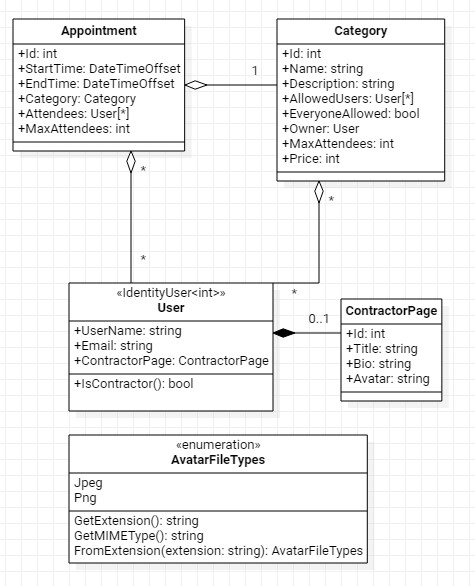
\includegraphics[width=0.8\textwidth]{entities_uml}
	\caption{Entitások UML diagrammja}
	\label{fig:entities}
\end{figure}

\clearpage

\subsubsection{DTO-k}
Az entitások mellett DTO\footnote{Data Transfer Object - Adatátviteli objektum}-kat is használtam, a REST API ezekkel az adatszerkezetekkel kommunikál kifelé. A fő különbségek a DTO-k és az entitások között, hogy az entitásokban objektumok tartalmazhatnak objektumokat, viszont mivel adat átvitel során ez lehet hogy fölösleges, ezért a DTO-kban csak az objektumok ID-je van eltárolva.

\begin{figure}[H]
	\centering
	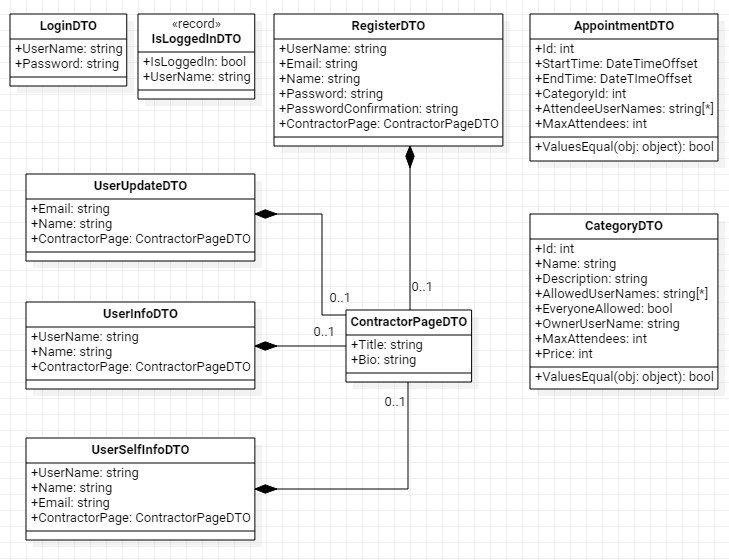
\includegraphics[width=1.0\textwidth]{dtos_uml}
	\caption{DTO-k UML diagrammja}
	\label{fig:dtos}
\end{figure}

\clearpage

\subsubsection{Logika}
A logikát megvalósító osztályaimat entitásonként különítettem el, azaz az egy fajta entitással dolgozó felhasználói esetek tipikusan egy osztályba kerültek. A logika osztályban lehet először látni a függőségi befecskendezés elvét. A logika osztályok csak a releváns repository-k interfészeit kapják meg.

\begin{figure}[H]
	\centering
	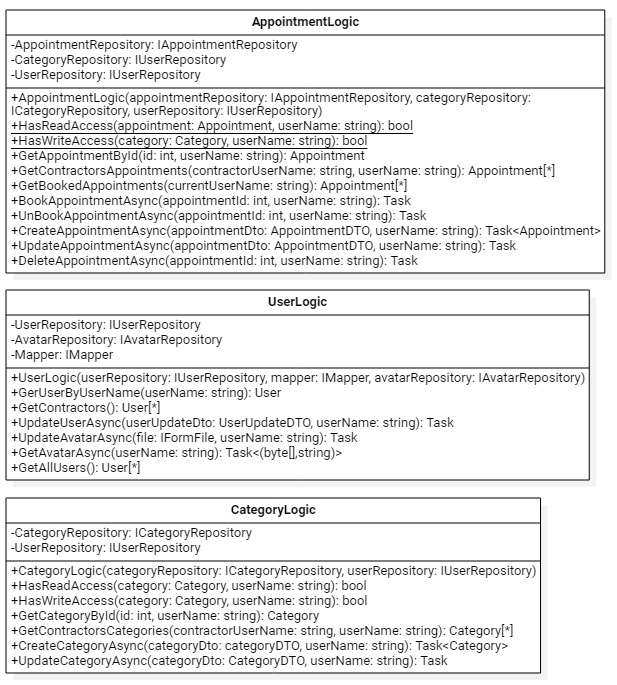
\includegraphics[width=1.0\textwidth]{logic_uml}
	\caption{Logika osztályok UML diagrammja}
	\label{fig:logic}
\end{figure}

\clearpage

\subsubsection{Kontrollerek}

A kontrollerek ugyan azokat a felhasználói eseteket fedik le, mint a logika osztályok. A különbség, hogy a bejövő HTTP kéréseket kezelik, alakítják át a logikának megfelelő adatra, utána meghívják a logika egy függvényét, majd a visszakapott belső reprezentációs adatot mappelik DTO-vá.

\begin{figure}[H]
	\centering
	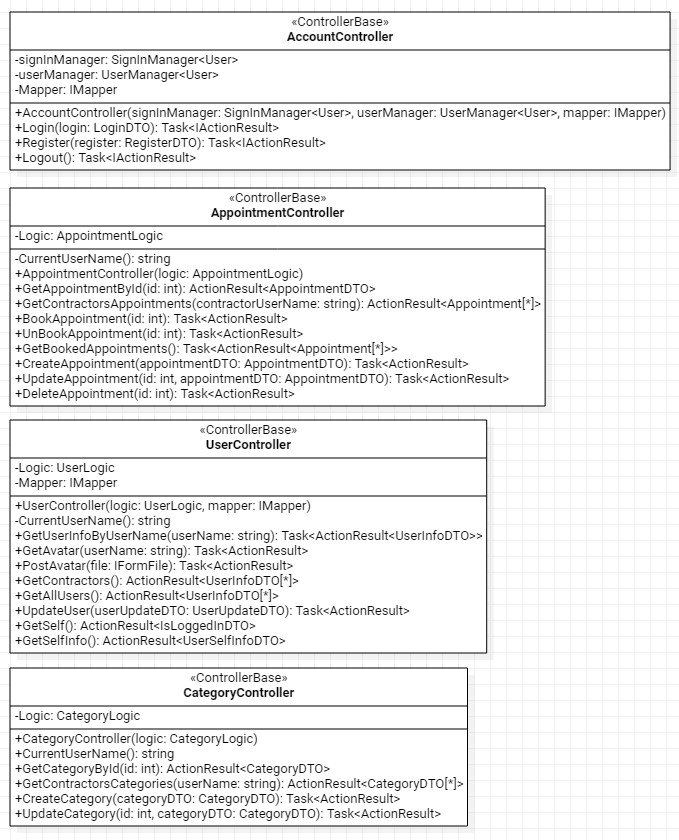
\includegraphics[width=1.0\textwidth]{controller_uml}
	\caption{Controller-ek UML diagrammja}
	\label{fig:controllers}
\end{figure}

\clearpage

\subsubsection{Repository-k}

Az adat elérő repository interfészek az alábbi \ref{fig:repoInterfaces} ábrán láthatók.
A repository megvalósítások nem képezik részét a diagrammnak, mert nem térnek el érdemben a megvalósított interfészektől, csak megvalósítjk azt.

\begin{figure}[H]
	\centering
	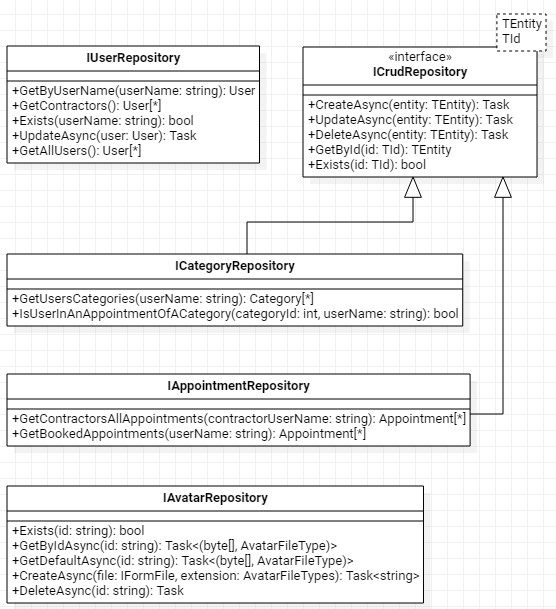
\includegraphics[width=1.0\textwidth]{repository_interface_uml}
	\caption{Repository interfészek UML diagrammja}
	\label{fig:repoInterfaces}
\end{figure}

\clearpage

\subsubsection{Program komponensek interakciója}

Mint látható, az entitásokon kívül az osztályok nem tartalmaznak állapot tárolásra szolgáló adattagokat. Ez a REST API állapotfüggetlensége miatt van. Így például a logika meg repository osztályok csak azért vannak osztályba szervezve, hogy ugyan azokat a befecskendezett függőségeket használják, hogy ne kelljen minden metódusuknál paraméterként megadni őket. Ettől funkcionális érzetű a kód, viszont ez a unit tesztelésnél hasznos, amit a \ref{sec:unittests} részben tárgyalok.

A program komponensei a következő módon függenek egymástól:

\begin{figure}[H]
	\centering
	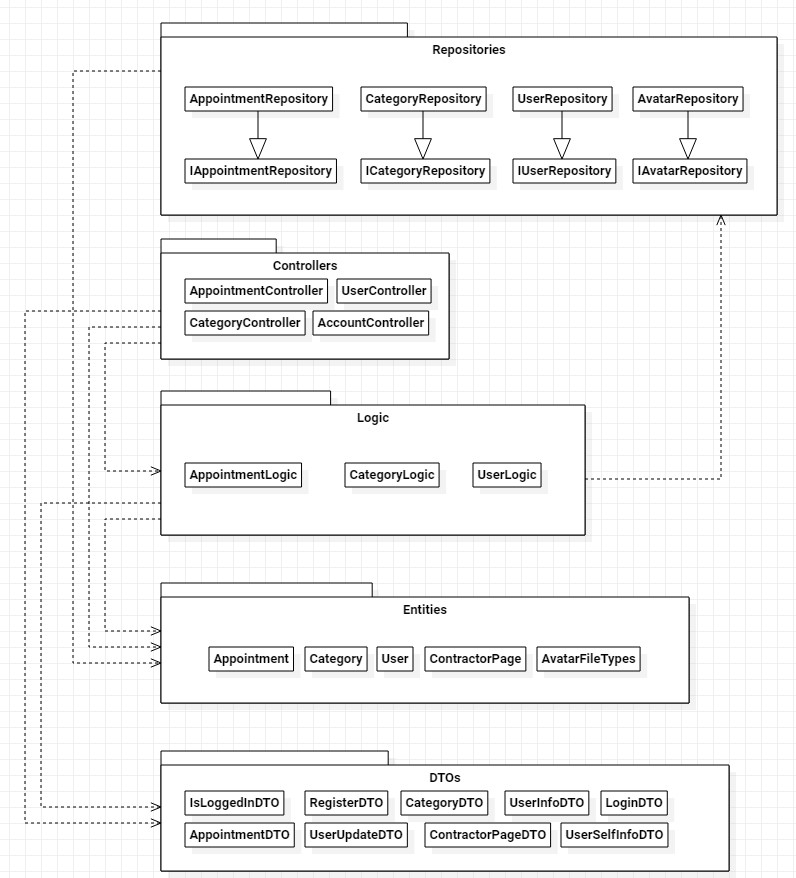
\includegraphics[width=1.0\textwidth]{package_uml}
	\caption{Program komponenseit összesítő UML diagramm}
	\label{fig:package}
\end{figure}

\todo{Szekvencia diagram egy példa requestnél}

\clearpage

\subsubsection{REST API végpontok}

A REST API végpontok a következőféleképpen néznek ki:

\begin{figure}[H]
	\centering
	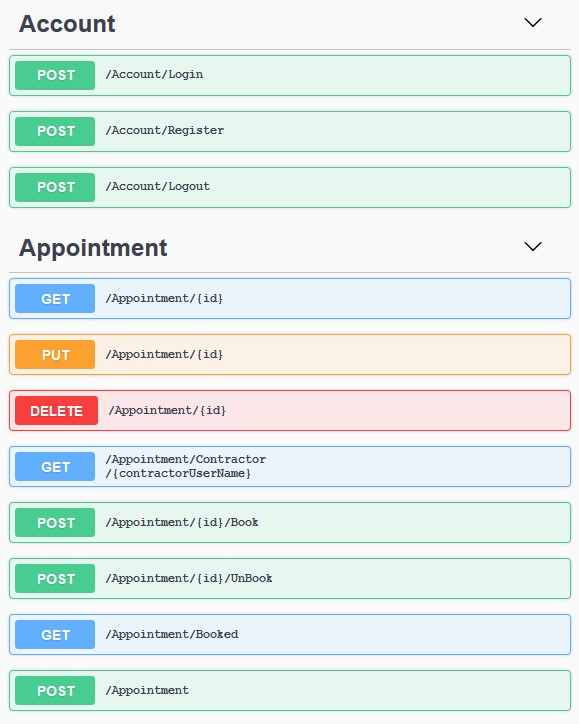
\includegraphics[width=0.9\textwidth]{api_doc_1}
	\caption{REST API végpontok}
	\label{fig:apiDoc1}
\end{figure}

\begin{figure}[H]
	\centering
	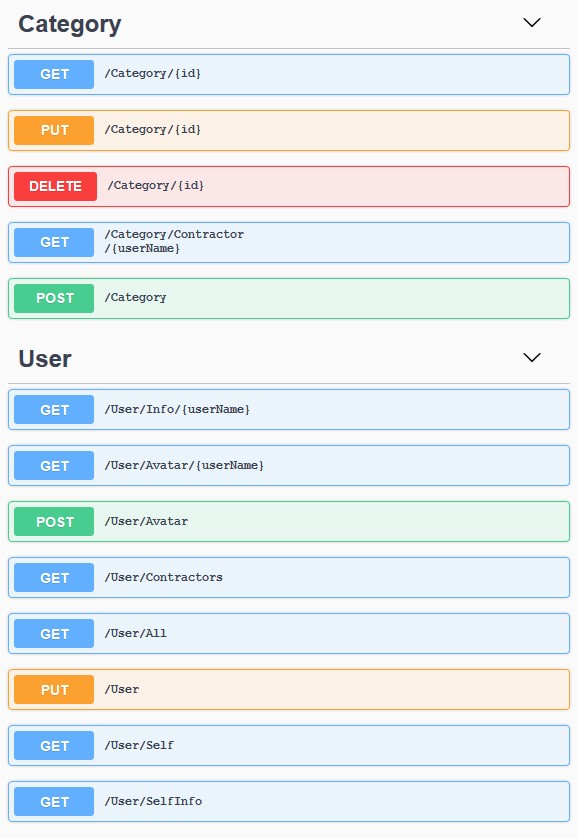
\includegraphics[width=0.9\textwidth]{api_doc_2}
	\caption{REST API végpontok folytatása}
	\label{fig:apiDoc2}
\end{figure}

\subsection{Adatbázis - Entity Framework}
Az Entity Framework\footnote{\url{https://docs.microsoft.com/en-us/ef/}} (továbbiakban EF) egy Microsoft által fejlesztett könyvtár a .NET-hez, egy ORM\footnote{Object-Relational Mapping - Objektum-Reláció fordítás} keretrendszer, mely C\# osztályokat fordít adatbázis elemekre és vissza. Code first módon elég a C\# osztályokat definiálni és az EF létrehozza az SQL táblákat és kapcsolatokat, a lekérdezéseket C\#-ban LINQ\footnote{\url{https://docs.microsoft.com/en-us/dotnet/csharp/programming-guide/concepts/linq/}} segítségével lehet végezni.

Azonban EF-el sem triviális az adatbázis kezelés, több a többhöz kapcsolatokat (pl.: egy ügyfél több időpontra is jelentkezhet és egy időpontra több ügyfél is jelentkezhet) elég sok manuális konfigurálással kell létrehozni, erről bővebben a megvalósítás \ref{sec:devProblems} részében írok.

Az adatbázis terve körülbelül egyezik az előző részben definiált entitásokkal, a következőképpen néz ki:

\todo{database uml}

Az EF-ben a DbContext osztály biztosítja az adat elérést és definíciót. A DbContext virtual DbSet propertyjei lesznek azok az értékek, amiket az EF használni fog. Az OnModelCreating metódusban lehet testre szabni, hogy hogyan is generálja le az objektumok között a kapcsolatok az EF. A backend DbContext-je az IWAContext a következőképpen néz ki:

\todo{iwacontext uml}


\subsection{Funkcionális Frontend}
\subsubsection{React és Typescript}

Az alkalmazás frontendjét React.js\footnote{https://reactjs.org/} keretrendszerrel Typescriptben valósítom meg. A Typescript kibővíti a Javascript nyelvet és típusellenőrzést biztosít fordítási időben. A Typescript fájlokat a fordító Javascript fájlokká fordítja, közben szintaktikai és szemantikai elemzéseket hajt végre.

A React keretrendszer alappillére, hogy komponensekből épül fel a felhasználói felület. Ezeket a komponenseket újra felhasználhatóra lehet tervezni, így kód duplikációt elkerülni. Meg van a lehetőség őket egymásba ágyazni, egymás között a komponenseknek kommunikálni, így komplex rendszereket lehet építeni relatíve kis építőelemekből.

A React a nevét a reaktivitásból kapta, a lényege, hogy dinamikusan változó felhasználói felületeket lehessen létrehozni, elkerülve a régi statikus, bármi változtatás után újra töltést igénylő oldalakat. Ezt egy virtuális DOM-al éri el, nem a böngészőre hagyja az oldal szerkezet kezelését, hanem Javascriptben kódban csinálja. Ennek az előnye, ha bármilyen érték változik és frissíteni kell a DOM elemeket, akkor a React el tudja dönteni, hogy konkrétan melyik elemeket kell újra rajzolni és csak azokat változtatja meg a böngésző DOM-jában, ezáltal nagyon gyors és hatékony.

React-ben régen osztály komponensekkel lehetett dolgozni, de újabban a funkcionális komponensek egyre több támogatást és funkciót kaptak, most már ez az ajánlott módja a React-ben való fejlesztésnek. A funkcionális komponensek lényege, hogy tiszta, mellékhatásmentes függvényekkel írjuk le a komponenseinket, melyek bemenetként kaphatnak bármilyen értéket és kimenetként a kirajzolandó komponenst adják vissza. Mivel ezek mellékhatásmentes függvények, ezért ha nem változik a bemenetük, akkor nem változik a kimenetük se, ezért a React nagyon effektíven tudja eldönteni, hogy állapot változásnál melyik komponenseket kell újra rajzolni és melyikeket nem.

Ennek ellenére valahogy mégis le kell kezelni például állapotok változását, külső API hívásokat, console-ra írást, melyeket tiszta környezetben nem tehetnénk meg. Erre adnak választ a React Hook-ok. Ezek a 'kampók' 'belekapaszkodnak' egy funkcionális komponensbe és a programozók oldalán egy funkcionális interfészt biztosít ilyen típusú dinamizmus kezelésére. A \textit{useState} hook például egy állapotot és egy állapot módosító függvényt biztosít nekünk. Egy gomb \textit{onClick} eseményében ha meghívjuk az állapot módosító függvényt, akkor a React a háttérben elvégzi nekünk az értékadást, mi csak azt vesszük észre, hogy az állapotunk megváltozott. Mivel a React kezébe adjuk mutálható változó értékek kezelését, ezért effektív tud maradni a keretrendszer, az előbb leírt feltételes újra rajzolásokat hatékonyan tudja kezelni.

\subsubsection{Async Result Monád típus}

Hibakezelésre imperatív programozási nyelvekben hagyományosan kivételeket használnak. Typescriptben is meg van a lehetősék kivételek dobására és elkapására. Viszont, mivel funkcionális komponensekkel dolgozok és fejlesztés közben párszor nem lekezelt kivételek miatt inkonzisztens állapotba került a UI, ezért a Haskellben \textit{Either} és Rust-ban \textit{Result} néven ismert monádhoz fordultam. Röviden ezeknek az a lényegük, hogy típus szinten kezeljük le a hibákat, amikor egy függvény alkalmazás lánc végén akarjuk használni az értéket, akkor muszáj megvizsgálnunk, hogy hibába ütköztünk-e vagy lefutott az összes számítás és felhasználhatjuk az értéket.

A Rust mintájára egy Result nevű unió típust\cite{tsUnionTypes} hoztam létre, ami egyszerre vagy egy Ok vagy egy Err osztályt tartalmazhat. Az Ok és Err is egy-egy értéket tartalmaznak, az Ok-ban szereplő érték egy jó értéket szimbolizál, amit utána tovább fel lehet használni, az Err pedig valamilyen hibát tartalmaz (pl.: string, Exception, saját osztály), mellyel nem folytatódik tovább a számítás.

A Result egy Funktor típus, definiálva van rá egy \textit{map} függvény. Hogy ha a Result Ok, akkor alkalmazza rá a függvényt, ha Err akkor pedig az Err-t adja vissza. Ezen felül a Result egy Monád típus, az \textit{andThen} függvény alkalmazza az Ok-ban levő értékre a függvényt ami egy Result típust ad vissza, vagy ha Err érték a Result, akkor visszaadja az Err-t. Az \textit{sideEffect} függvénnyel mellékhatásosságot lehet elérni, a Result marad ugyan az, viszont az Okban levő értékére lehet mellékhatásos függvényeket hívni. Ez azért hasznos, mert a Javascriptet nem tisztán funkcionálisra tervezték és például a böngésző API-jával való kommunikációhoz hasznos lehet.

Result-ból adatot kinyerni a \textit{match} függvénnyel lehet, ami paraméterül kap egy Ok esetén és egy Err esetén lefutó függvényt, a Result értéke szerint a megfelelőt futtatja le.

Kivételt dobó függvényeket be lehet csomagolni, hogy Result-ot adjanak vissza a \textit{fromThrowable} függvénnyel. Ha egy függvény nem dob kivételt, de mégis szeretnénk, hogy Result-ba csomagolt visszatérítési értéke legyen, akkor a \textit{fromSafe} függvénnyel tehetjük meg.

Javascritben és ezáltal Typescriptben az aszinkron függvényeknek muszáj Promise típussal visszatérniük. Ez megnehezíti a dolgunkat, mert például Result típust így nem tudunk visszaadni. Ezt a problémát oldja meg a ResultPromise, ami lényegében egy Result-ba csomagolt Promise. Ugyan azokkal a függvényekkel rendelkezik mint a Result (\textit{map}, \textit{andThen}, \textit{sideEffect}), viszont Promise-okkal dolgozik a háttérben. Ha egy Promise Rejected állapotba kerülne, akkor a ResultPromise-on belüli Result Err lesz.

A Result függvények amik Async végződésűek ugyan azon az elven alapulnak, mint a megfelelőik (pl.: \textit{map}, \textit{mapAsync}) csak aszinkron függvényekkel dolgoznak.

Összességében, a Result és ResultPromise típusokkal és függvények kompozíciójával sok hibakezelő boilerplate kód kerülhető el és típus biztos lehet a kód.

\subsubsection{Logika}

Az entitások és a DTO-k egyeznek a \ref{fig:entities} és \ref{fig:dtos} ábrák UML diagrammjaival. Ez azért célszerű, mert így ugyan azon belső reprezentációval tudunk dolgozni front és backenden is.

Frontend logikához tartozik a \textit{reportGenerator} és a \textit{pdfReportGenerátor modul}. Az előbbi adott időpontokból generálja le a számla adatait, az utóbbi pedig PDF-et generál belőle. A PDF készítés így a frontenden történik, ehhez a PDFMake könyvtárat használtam. Ebben egy sajátos adatszerkezetben kell definiálni a PDF tartalmát és stílusát, a PDFMake dokumentációjában\footnote{\url{https://pdfmake.github.io/docs/0.1/}} erről lehet bővebben olvasni.

\subsubsection{Repository-k}

A fronetenden is a backendhez hasonlóan az adatelérést repository osztályokba és interfészekbe szerveztem, azzal a különbséggel, hogy itt a REST API-n keresztül éri el az adatot. A repositoryk struktúrája egyezik az API végpontokkal, melyek a \ref{fig:apiDoc1} és \ref{fig:apiDoc2} ábrákon találhatók.

A repository-k a ResultPromise típust használják, a \textit{safeApiFetch} függvény valamelyik változatával. Ez a függvény család a Javascript-es fetch függvényt csomagolja ResultPromise típusba, a függvényhívás után ha nem 2** a státusz kód akkor Err-t adnak vissza, az \textit{As} függvények jó érték esetén transzformálják az adatot megfelelő alakra. 

\subsubsection{Hook-ok}

A \textit{Status} típus egy unió tíups, ami vagy Idle, Loading, Failed valamilyen értékkel vagy Loaded valamilyen értékkel. Ez lehetővé teszi, hogy egy API hívás állapotát láthassuk, a felhasználói felületen ennek megfelelően rajzoljuk ki a kompknenseket.

A \textit{useApiCall} hook egy API hívást tud végrehajtani, visszatérési értékként visszaadja a hívás jelenlegi állapotát Status-ban és egy callback függvényt, aminek a meghívásával lefut az API hívás. A komponensekben legtöbb esetben ezzel a useApiCall hook-al érem el az API-t.

A \textit{useLogin} hook ugyan úgy működik mint a \textit{useApiCall} viszont egy sikeres API hívás után bejelentkezteti a felhasználót. A \textit{useLogout} hasonló, csak kijelentkezteti a felhasználót és visszairányítja a főoldalra.

A \textit{useCookieLogin} a callback hívásánál megnézi, hogy be van-e jelentkezve jelenleg az alkalmazásba a felhasználó, ha nincs, akkor egy API call-al elküldi a backendnek, hogy cookie alapján bejelentkezhet-e, ha igen, akkor cookie alapján bejelentkezteti a felhasználót. A useCookieLogin lefut az alkalmazás betöltése előtt, azért, hogy már alapból úgy töltsön be az alkalmazás, hogy a felhasználó be van jelentkezve.

\subsubsection{Kontextusok}

A React kontextusok lényege, hogy több komponens ugyan ahhoz az adathoz hozzá tudjon férni, de ne kelljen paraméternek mindig átadni az adott értékeket. Például ha egy komponensen belül több komponens van amin belül még vannak komponensek, akkor mindegyiknek paraméternként kellene átadni az adatot, így viszont egy közös kontextusból elérhetik.

A \textit{DIContext} egy nagyon egyszerű függőségi befecskendezés implementáció, a komponensek a kontextuson keresztül érhetik el a nekik megfelelő függőségeket, amik vagy repository-k vagy a konfigurációs osztály.

A \textit{LoginProvider} tartalmazza azt, hogy a felhasználó be vagy ki van jelentkezve és lehetőséget ad a bejelentkezett státus megváltoztatására.

A \textit{NotificationProvider} felel a különböző értesítések kezeléséért. A \textit{notificationDispatch} függvényével lehet hibákat, felszólításokat és sikeres értesítéseket hozzáadni a megjelenítéshez, utána a NotificationProvider ezek alapján rajzolja ki az értesítéseket a \textit{Notification} komponens segítségével.

A \textit{DataProvider} entitások listáját tudja szolgáltatni a komponenseknek. Így például egy oldalon a vállalkozó kategóri és időpontjai lehet számon tartva, a \textit{dataDispatch} függvényen keresztül változatni. Például a foglalás gomb miután elküldte a foglalási kérést a backendnek a frissült időpontot frissíti a DataContext-ben is. A \textit{dataDispatch}-nél a leglátványosabb, hogy a kontextus adatát  React Reducer-el valósítom meg, ami egy immutable állapot változtatás. A többi kontextusban is használom, viszont itt szerepel a legtöbb funkcionális nyelvi elem. 

\subsubsection{Komponensek}

AppointmentCard, AppointmentAgenda, CategoryCard

DatePicker, UserSelector

Modal, Editorbase, User/Appointment/Category editor, UserAdder, AppointmentViewer, CategoryViewer

\clearpage

\section{Megvalósítás}
\subsection{Fejlesztési környezet}

Fejlesztői környezetnek eleinte Microsoft Visual Studio 2019\footnote{\url{https://visualstudio.microsoft.com/}}-et használtam a backend C\# kód írásához, a frontendhez pedig Visual Studio Code\footnote{\url{https://code.visualstudio.com}}-ot. Ezek teljes funkcionalitású fejlesztői környezetek, mindent képesek voltak nyújtani ami a fejlesztéshez szükséges volt. Viszont időközben JetBrains Rider\footnote{\url{https://www.jetbrains.com/rider/}}-re váltottam, egyrészt azért, mert a Visual Studio-val ellentétben cross-platform, másrészt mert a JetBrains IDE-k egymás között tudnak funkcionalitást használni, így volt TypeScript nyelv támogatás, ezzel egy IDE-t kellett csak használnom.

Verziókövetésre Git\footnote{\url{https://git-scm.com/}}-et, a konténerizációhoz Docker-t használtam.

A backend-hez .NET 5\footnote{\url{https://dotnet.microsoft.com/download/dotnet/5.0}}-öt használtam C\# 9-el. A .NET csomagkezelő rendszere a NuGet, a következő NuGet csomagokat használtam az ASP.NET keretrendszerhez szükségeseken kívül:

\begin{compactitem}
	\item XUnit: Egységtesztelést segítő csomag
	\item AutoMapper: Objektum map-elést automatizáló csomag
	\item Moq: Egységteszteknél a mock-olás eléréséhez szükséges csomag
	\item Coverlet: Teszt lefedettség generálásához szükséges csomag
\end{compactitem}

A frontend Node.js\footnote{\url{https://nodejs.org/en/}}-t, TypeScript-et, React.js-t használ. Csomag kezelőnek Yarn\footnote{\url{https://yarnpkg.com/}}-t, build eszköznek és bundler-nek Snowpack\footnote{\url{https://www.snowpack.dev/}}-et használtam. Ezeken kívül a következő csomagokat használja a frontend:

\begin{compactitem}
	\item Jest: JavaScript teszt keretrendszer
	\item Luxon: Dátum és idő kezelő könyvtár
	\item Pdfmake: Böngészőben PDF generáló könyvtár
	\item React Router: SPA\footnote{Single Page Application - Egy oldalas alkalmazás, a linkek nem egy új lapot töltenek be, hanem a javascript változtatja meg az oldal tartalmát az újra}-hoz szükséges routing könyvtár
	\item React Select: Lenyíló lista komponens React-hez
	\item uuid: GUID\footnote{Globally Unique Identifier - Teljesen egyedi azonosító} létrehozó könyvtár
\end{compactitem}

A frontend kódot a \textit{yarn build} paranccsal lehet legenerálni. A \textit{yarn dev} parancs elindítja a fejlesztői környezetet, azaz egy élőben fájl változásokra újratöltő webszervert indít a http://127.0.0.1:8100 címen. A \textit{yarn test} parancs lefuttatja a frontend tesztjeit.


\subsection{Fejlesztési döntések}
Fejlesztés közben a következő döntéseket hoztam, hogy a tervezett kód egyszerűbben legyen implementálható.

Létrehoztam saját kivételeket backend-en, amiket így különböző szituációkban le lehet kezelni, ezek:

\begin{compactitem}
	\item NotFoundException: Egy adott elem nem található.
	\item UnauthorisedException: A kért felhasználó nem férhet hozzá egy entitáshoz
	\item InvalidEntityException: Egy entitásnak nem teljesül az objektum invarianciája.
	\item AlreadyBookedException: Egy időpontot már előbb lefoglalt a felhasználó.
	\item NotBookedException: Egy időpontot ezelőtt nem foglalt le a felhasználó.
	\item InvalidAvatarFileException: A profilkép nem megfelelő.
	\item NotContractorException: Egy felhasználó nem vállalkozó.
\end{compactitem}

A DTO-k és entitások közötti konverziót Mapper osztályokkal kiviteleztem. A triviális mappeléseket az AutoMapper könyvtárral implementáltam. A komplexebb osztályokra mint az Appointment és Category saját Mapper-t írtam, ezek az AppointmentMapper és CategoryMapper.

A C\# 9 újonnan bevezetett nyelvi elemét, a rekord típusokat, is sok helyen használtam a kódomban. A record típusokkal előre megírt funkcionalitást kaphatunk egy objektumra, például property-k alapján érték szerinti egyenlőséget és immutability-t. Mivel a DTO és entitás osztályaim csak adatot tárolnak, ezért itt ki tudtam használni ezeket a funkciókat.

Főleg a repository-knál kihasználtam a LINQ\footnote{LINQ - Language Integrated Query} könyvtárat, ezzel felsoroló objektumokból funkcionális stílusú kóddal tudtam adatokat szűrni, rendezni és manipulálni.

\subsection{Fejlesztés közben felmerült problémák}
\label{sec:devProblems}
Fejlesztés közben több nem triviális probléma is merült fel, ezeket részletezem most, hogy későbbi fejlesztésnél lehessen ezekre hivatkozni, elkerülni őket.

\subsubsection{EF virtual nullable}

Az EF-nél fontos, hogy ha egy entitásunk egy másik entitásra hivatkozik, akkor azt az adattagot virtuálisként deklaráljuk, ez a keretrendszer megkötése. Így tudja elérni az EF, hogy a háttérben lusta betöltéssel tudja az adatbázisból elérni optimális módon az adatokat, leörököl az osztályból és a virtuálisság miatt felülírja a saját lusta kiértékelésű implementációjával a betöltést.

Nullable típusok mellett, hogy ha nem adunk meg az adattagjainknak kezdő értéket, akkor a fordító szól érte. Ezt a \textbf{null!} segítségével lehet megoldani. A \textbf{!} operátor a típusellenőzrőnek ad egy biztosítást, hogy mi itt biztosan tudjuk, hogy az értékünk nem lesz null, a programozó ellenőrizte. Jelen esetben az EF-nél biztosan nem lesz null az adott érték, mert az EF betölti az adatbázisból, viszont a konstruktorban muszáj neki értéket adni, ezt oldja meg a \textbf{null!}.

\subsubsection{EF many-to-many}

Az EF alapból támogatja a több a többhöz adatbázis kapcsolatokat, például az alkalmazásban több felhasználó foglalhat egy időpontot és egy időpontra több felhasználó is lehet résztvevő. Valamiért ezt a kapcsolatrendszert az EF nem tudta lekezelni, egy időpontra csak egy felhasználót engedett.

Ezt a problémát kapcsolótáblákkal oldottam meg. Ez azt jelenti, hogy különböző kapcsoló objektumokat kellett létrehozni (AttendeeOnAppointments, AllowedUserOnCategories) és ezeket a különböző összekapcsolandó entitásokra egy listába (pl.: AttendeeOnAppointmentsJoin, OwnerOfCategories).

Ahhoz, hogy az EF ezeket használni tudja, a DbContext OnModelCreating metódusát felül kell írni és a ModelBuilder megfelelő függvényeivel konfigurálni, ez a kódban látható.

\subsubsection{Integrációs tesztek párhuzamosítása}

Az EF mellé integrációs teszteknél egy memóriában futó SQL szervert szoktak használni. Ennek az előnye, hogy nem kell egy külső SQL szervert használni ami lemezre ír, hanem eldobható és nagyon gyors. Ezekkel voltak problémák fejlesztés közben, ezért SQLite in-memory adatbázisra álltam át, ezt a \ref{sec:integrationTests} részben részletezem.

Fejlesztés közben felmerült az a probléma, hogy a tesztek valamiért ugyan ahhoz az adatbázis példányhoz fértek hozzá. Ezt azért nem célszerű, mert így amikor az egyik teszt törölt az adatbázisból, akkor a másik nem tudta kiolvasni a megfelelő értékét. A unit és integrációs teszteknek mindig környezetfüggetlennek kell lenniük, nem szabad két teszt futtatásnak befolyásolnia egymást.

Erre az volt a megoldás, hogy az SQLite keepalive conneciton-t minden teszt destruktorában be kell zárni. Ezzel a tesztek párhuzamosíthatók lettek és nem akadtak össze, a futási idejük is nagyon lecsökkent.

\section{DevOps}
\subsection{CI/CD}
Fejlesztéshez Github\footnote{\url{https://github.com/}}-ot használtam, ez a Git verziókövető rendszernek egy online kód tárolója és kollaborációs platformja. Bár a szakdolgozatomban a kollaborációs lehetőségeket nem használhattam ki, a projektmenedzsment eszközök hasznosak voltak.

A Github lehetőséget biztosít Continous Integration (röviden CI) és Continous Deployment (röviden CD) használatára a Github Actions-ön belül. A CI lényege, hogy amikor egy új változtatás kerül fel Github-ra, akkor automatikusan le tudja fordítani és tesztelni a kódot, esetleg különböző elemzéseket vagy dokumentációt tud generálni. Ezzel megfelelő tesztelési lefedettség mellett lehet garantálni, hogy ha hibák kerülnének a programba, akkor azokat hamar észre vegyük.

A CD lényege, hogy a változtatott kódot és frissített alkalmazást minél többször és gyorsabban lehessen megjelentetni, kihelyezni. \todo{Ha lesz CD akkor azt ide kifejteni}Az én alkalmazásomban végül időhiány miatt ezt nem implementáltam, de a modern fejlesztői környezet és dockerizált architektúra miatt a jövőben meg lehetne valósítani. A gyakorlatban ez úgy nézne ki, hogy vagy a master branch-be minden commitnál, vagy minden éjszaka, a CI lefordítja és leteszteli a kódot. Ha nem talál benne hibát, akkor a CD megépíti a Docker konténereit az alkalmazásnak amit utána egy egyszerű script-tel kihelyez a szerverre. Ezt például úgy teheti meg, hogy a szerveren levő Docker letölti ezt a frissebb konténert és lecseréli a jelenleg futót.

A jelenlegi CI konfiguráció a \textit{.github/workflows} mappában található.

\subsection{Docker}
A Docker egy konténerizációs technológia, amely megkönnyíti az alkalmazások kihelyezését. Az alkalmazások 'konténerekbe' csomagolódnak minden függőségükkel, ezen konténereket utána egy egységként lehet futtatni, nem kell a felhasználó rendszerére egyesével a program futásához felállítani a környezetet.

A Docker konténereket úgy találták ki, hogy eldobhatók legyenek, azaz ki lehessen őket törölni és újra futtatni és ugyan úgy működjenek. Az adatok perzisztálását így \textit{volume}-okkal oldhatjuk meg, jelen esetben az adatbázis és a profilképeket a host gép lokális mappáiban tároljuk.

Egy konténer adatait egy Dockerfile nevű fájlban definiálhatjuk. Itt megadhatjuk, hogy milyen más image-ből szeretnénk kiindulni (pl.: ubuntu, debian, node.js, dotnet) és utána, hogy azt hogy szeretnénk testre szabni. Az én Dockerfile-jaim használnak \textit{builder}-eket, ami azt jelenti, hogy az elején definiálom, hogy a forráskód milyen környezetben legyen lefordítva, utána pedig egy másik környezetet definiálok, amiben azt a lefordított kódot futtatom. Ennek az az előnye, hogy a végleges futtatható konténerben nincsenek fordításhoz szükséges függőségek, így kisebb a konténer mérete.

\subsubsection{Konténerek optimalizálása}

A konténereimben Alpine Linux\footnote{https://alpinelinux.org/}-ot használok. Az Alpine egy minimális Linux disztribúció, melynek a konténerekre optimált változata <3MB. Ezzel szemben egy Ubuntu vagy Debian alapú konténer csak a disztribúciók miatt több száz MB is lehet.

Egy Docker konténer buildelése közben a Docker megjegyzi, hogy az egyes utasításokat ugyan ilyen környezetben végrehajtotta-e már, ha igen, akkor az elcache-elt értéket használja. Ez azt jelenti, hogy ha a konténerünk elején telepítünk fordításhoz szükséges programokat, akkor a következő buildnél nem fogja még egyszer feltelepíteni őket nulláról, hanem használja az előző build cache-ét. Ezt a cache-t a COPY felrúghatja, amikor a fájlrendszerünkről másolunk a konténerbe fájlokat. Ezek a fájlok változhatnak builek között, így nem biztos, hogy lehet cache-elni. A Docker ezeket a fájlokat hash-eli és összehasonlítja, ha nem változtak akkor használja a cache-t. Ez a gyakorlatban azért jó, mert például a frontendél a sok npm csomag sokáig települ. Ha a konténerbe bemásolom csak a \textit{package.json} és \textit{yarn.lock} fájlokat és hívom meg a \textit{yarn install} parancsot, akkor ha a következő konténer buildnél nem változnak a dependency-k, akkor lehet cache-ből betölteni azokat. Ez által fejlesztés közben gyorsítható a buildelés folyamata.

\subsubsection{Docker Compose}

A Docker Compose programmal konténereket lehet orkersztrálni, egy konfigurációs fájlban eltárolni, hogy ezek milyen környezeti változókat, fájlokat, portokat használhatnak, egymást hogy érik el. Mivel egy fájlban található ez a konfiguráció, egyszerűsíti egy teljes rendszer feltelepítési és üzemeltetési komplexitását.

Az alkalmazásban így például a MariaDB adatbázist deklaráltam egy konténernek, megadtam, hogy a backend azt érje el, így az adatbázis telepítése és üzemeltetése is nagyon egyszerű.

\section{Tesztelés}

Mind az integrációs, mind a unit teszteknél a következő struktúrát használtam. Létrehoztam egy teszt osztályt a tesztelendő osztálynak (logika, repository, mapper). Ezen belül létrehoztam egy osztályt a függvény / metódus nevével, azon belül pedig a függvények nevei az adott esetet írják le. Például, sikeres, nem engedélyezett felhasználó, már lefoglalt időpont.

\begin{figure}[H]
	\centering
	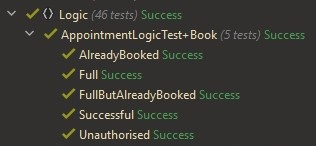
\includegraphics{test-naming}
	\caption{Teszt struktúra}
\end{figure}

\todo{screenshot, hogy lefutott az összes teszt}

\subsection{Unit tesztek}
\label{sec:unittests}
Unit tesztelésnél a backend logika, mapper és repository implementációk függvényeit teszteltem white box módon.

Tesztelésnél sokat segített a függőségi befecskendezés és az úgynevezett mock-olás. Mockolsánál létrehozunk egy hamis interfész implementációt, ez után különböző szabályokkal megadhatjuk, hogy melyik függvények milyen paraméterekre milyen értékeket adjanak vissza.

Például az AppointmentLogic CreateAppointment metódusában meghívom a CategoryRespoitory GetById metódusát és az AppointmentRepository CreateAsync metódusát. Ha mockolom a CategoryRepository-t, akkor megmondhatom, hogy ha a GetById-t 10-re hívják meg, akkor adjon vissza egy konkrét kategóriát amit előtte definiálok. Az AppintmentRepository-nál pedig a mockolás miatt ellenőrizni tudom, hogy sikeres futás után meghívta-e a logika pontosan egyszer a CreateAsync metódust.

Ezzel a unit tesztjeim futásai közben nem kell futnia az adatbázisnak, mert a repository-k nem az adatbázisban dolgoznak, hanem a mockolt objektummal váltottam ki a működésüket. Viszont, a logika szempontjából ugyanúgy egy repository-n keresztül dolgozunk, a logika teljesen jól tesztelhető, nem függ külső szolgáltatásoktól.

A repository-k teszteléséhez hasonlóan mockolok, viszont az EF DbContext-jét kell mockolni, azon keresztül érhető el az adatbázis. Erre a MockDbContextBuilder osztály szolgál, ami létrehoz egy mock DbContext-et a szolgáltatott adatokkal. Így azt lehet szimulálni, hogy azok az adatok vannak az adatbázisban, lehet tesztelni a repository helyességét, hogy megfelelően kérdezi le vagy módosítja őket.

A kontrollereket nem unit tesztelem, mert csak átalakítják a bemenetet, meghívják a logika egy függvényét és DTO-vá alakítják a kimenetet. A kontrollereket integrációs tesztelés során tesztelem, mert ha az integrációs tesztek átmennek, akkor az azt jelenti, hogy a kontrollerek is jók.

Az unit tesztek a következő struktúrájúak:
\begin{enumerate}
	\item \textbf{Arrange:} A teszthez szükséges adatok előkészítése. Itt általában a mock objektumok előkészítése történik, vagy a várt eredmény definiálása.
	\item \textbf{Act:} A tesztelendő műveletek végrehajtása, a visszatért érték eltárolása egy változóban. Kezelt kivételek esetén azt ellenőrzöm, hogy kiváltódott-e a megfelelő kivétel.
	\item \textbf{Assert:} Ellenőrzés, hogy a művelet megfelelően hajtódott-e végre. Ellenőrzöm a visszatérési érték helyességét és azt, hogy a mock objektum megfelelő metódusai megfelelően meg lettek-e hívva vagy nem.
\end{enumerate}

\subsection{Integrációs tesztek}
\label{sec:integrationTests}
A backendem integrációs tesztelve is lett. Ez azt jelenti, hogy az api-t futtatom és nem egyesével az egységeit tesztelem mint unit tesztelésnél, hanem hogy az egész rendszer a bejövő kéréstől a kiadott válaszig jól működik-e.

Ahhoz, hogy az integrációs tesztek gyorsak és külső szolgáltatás függetlenek legyenek SQLite\footnote{\url{https://www.sqlite.org}} inmemory adatbázist használok. Ez egy teljes értékű SQL szerverrel ér fel, ami az eszköz memóriájában fut. Így az integrációs futhatnak Coninous Integration közben, nem kell egy MardiaDB szervert futtatni a felhőben.

Az integrációs tesztekhez egy előre elkészített adat csomagot töltök be mindig az adatbázisba, ezt az IntegrationTestData osztály tartalmazza.

A TestWebApplicationFactory egy gyár tervmintát alkalmazó osztály, ami az előbb említett SQLite imemory adabázzissal konfigurál fel és készít el egy alkalmazás példányt.

Az IntegrationTestBase osztály az ősosztálya az összes integrációs teszt osztálynak, tartalmaz egy TestWebApplicationFactory-t és pár segédfüggvényt, hogy egyszerűbb legyen megírni a teszteseteket.

Az integrációs tesztek a következő struktúrájúak:
\begin{enumerate}
	\item \textbf{Arrange:} A teszthez szükséges adatok előkészítése. Ez lehet egy új DTO létrehozás, amit majd egy POST request-el elküldök az API-nak, vagy az adatbázisból érték kiolvasás, hogy a végén össze lehessen hasonlítani, hogy egyezik-e a visszatért értékkel.
	\item \textbf{Act:} A tesztelendő műveletek végrehajtása. Egy HTTP klienssel HTTP kéréseket küldök az API-nak, ha kell egy DTO-val, vagy előtte még egy bejelentkező kéréssel.
	\item \textbf{Assert:} Ellenőrzés, hogy a műveletek megfelelően hajtódtak-e végre. Itt vizsgálom a HTTP státusz kód helyességét, a visszatért JSON adatot beolvasom DTO-ként és ellenőrzöm, hogy megfelelő-e.
\end{enumerate}

\subsection{Manuális tesztek}
frontend tesztelés
























% Lorem ipsum dolor sit amet, consectetur adipiscing elit. Duis nibh leo, dapibus in elementum nec, aliquet id sem. Suspendisse potenti. Nullam sit amet consectetur nibh. Donec scelerisque varius turpis at tincidunt.


% \section{Tételek, definíciók, megjegyzések} % Theorem-like items

% \begin{definition}
% Mauris tristique sollicitudin ultrices. Etiam tristique quam sit amet metus dictum imperdiet. Nunc id lorem sed nisl pulvinar aliquet vitae quis arcu. Morbi iaculis eleifend porttitor.
% \end{definition}

% Maecenas rutrum eros sem, pharetra interdum nulla porttitor sit amet. In vitae viverra ante. Maecenas sit amet placerat orci, sed tincidunt velit. Vivamus mattis, enim vel suscipit elementum, quam odio venenatis elit, et mollis nulla nunc a risus. Praesent purus magna, tristique sed lacus sit amet, convallis malesuada magna. Phasellus faucibus varius purus, nec tristique enim porta vitae.

% \begin{theorem}
% Nulla finibus ante vel arcu tincidunt, ut consectetur ligula finibus. Mauris mollis lectus sed ipsum bibendum, ac ultrices erat dictum. Suspendisse faucibus euismod lacinia. Etiam vel odio ante.
% \end{theorem}
% \begin{proof}
% Etiam pulvinar nibh quis massa auctor congue. Pellentesque quis odio vitae sapien molestie vestibulum sit amet et quam. Pellentesque vel dui eget enim hendrerit finibus at sit amet libero. Quisque sollicitudin ultrices enim, nec porta magna imperdiet vitae. Cras condimentum nunc dui.
% \end{proof}

% Donec dapibus sodales ante, at scelerisque nunc laoreet sit amet. Mauris porttitor tincidunt neque, vel ullamcorper neque pulvinar et. Integer eu lorem euismod, faucibus lectus sed, accumsan felis. 

% \begin{remark}
% Nunc ornare mi at augue vulputate, eu venenatis magna mollis. Nunc sed posuere dui, et varius nulla. Sed mollis nibh augue, eget scelerisque eros ornare nec. Praesent porta, metus eget eleifend consequat, eros ligula eleifend ex, a pellentesque mi est vitae urna. Vivamus turpis nunc, iaculis non leo eget, mattis vulputate tellus.
% \end{remark}

% Fusce in aliquet neque, in pretium sem. Donec tincidunt tellus id lectus pretium fringilla. Nunc faucibus, erat pretium tempus tempor, tortor mi fringilla neque, ac congue ex dui vitae mauris. Donec pretium et quam a cursus.

% \begin{note}
% Aliquam vehicula luctus mi a pretium. Nulla quam neque, maximus nec velit in, aliquam mollis tortor. Aliquam erat volutpat. Curabitur vitae laoreet turpis. Integer id diam ligula.
% \end{note}

% Ut sollicitudin tempus urna et mollis. Aliquam et aliquam turpis, sed fermentum mauris. Nulla eget ex diam. Donec eget tellus pharetra, semper neque eget, rutrum diam.

% \subsection{Egyenletek, matematika} % Equations, formulas

% Duis suscipit ipsum nec urna blandit, $2 + 2 = 4$ pellentesque vehicula quam fringilla. Vivamus euismod, lectus sit amet euismod viverra, dolor metus consequat sapien, ut hendrerit nisl nulla id nisi. Nam in leo eu quam sollicitudin semper a quis velit.

% $$a^2 + b^2 = c^2$$

% Phasellus mollis, elit sed convallis feugiat, dolor quam dapibus nibh, suscipit consectetur lacus risus quis sem. Vivamus scelerisque porta odio, vitae euismod dolor accumsan ut.

% In mathematica, identitatem Euleri (equation est scriptor vti etiam notum) sit aequalitatem Equation~\ref{eq:euler}:
% \begin{equation}\label{eq:euler}
% e^{i \times \pi} + 1 = 0
% \end{equation}


% \section{Forráskódok} % Source code samples

% Nulla sodales purus id mi consequat, eu venenatis odio pharetra. Cras a arcu quam. Suspendisse augue risus, pulvinar a turpis et, commodo aliquet turpis. Nulla aliquam scelerisque mi eget pharetra. Mauris sed posuere elit, ac lobortis metus. Proin lacinia sit amet diam sed auctor. Nam viverra orci id sapien sollicitudin, a aliquam lacus suscipit. Quisque ac tincidunt leo Code~\ref{src:cpp} and \ref{src:csharp}:

% \lstset{caption={Hello World in C++}, label=src:cpp}
% \begin{lstlisting}[language={C++}]
% #include <stdio>

% int main() 
% {
% 	int c;
% 	std::cout << "Hello World!" << std::endl;

% 	std::cout << "Press any key to exit." << std::endl;
% 	std::cin >> c;
	
% 	return 0;
% }
% \end{lstlisting}

% \lstset{caption={Hello World in C\#}, label=src:csharp}
% \begin{lstlisting}[language={[Sharp]C}]
% using System;
% namespace HelloWorld
% {
% 	class Hello 
% 	{
% 		static void Main() 
% 		{
% 			Console.WriteLine("Hello World!");
			
% 			Console.WriteLine("Press any key to exit.");
% 			Console.ReadKey();
% 		}
% 	}
% }
% \end{lstlisting}

% \subsection{Algoritmusok} % Algorithms

% A general Interval Branch and Bound algorithm is shown in Algorithm~\ref{alg:ibb}. One of the following selection rules is applied in Step \ref{step:selrule}.\\
% Példa forrása: \href{https://www.inf.u-szeged.hu/actacybernetica/}{Acta Cybernetica (ez egy link)}.

% \begin{algorithm}[H]
% \caption{A general interval B\&B algorithm} 
% \label{alg:ibb} 
% \textbf{\underline{Funct}} IBB($S,f$)
% \begin{algorithmic}[1] % sorszámok megjelenítése minden n. sor előtt, most n = 1
% \STATE Set the working list ${\cal L}_W$ := $\{S\}$ and the final list ${\cal L}_Q$ := $\{\}$     
% \WHILE{( ${\cal L}_W \neq \emptyset$ )} \label{alg:igoend}
% 	\STATE  Select an interval $X$ from ${\cal L}_W$ \label{step:selrule}\COMMENT{Selection rule}  
% 	\STATE Compute $lbf(X)$ \COMMENT{Bounding rule}		  
% 	\IF[Elimination rule]{$X$ cannot be eliminated}
% 		\STATE Divide $X$ into $X^j,\ j=1,\dots, p$, subintervals   \COMMENT{Division rule}
% 		\FOR{$j=1,\ldots,p$}
% 			\IF[Termination rule]{$X^j$ satisfies the termination criterion}
% 				\STATE Store $X^j$ in ${\cal L}_W$ 
% 			\ELSE
% 				\STATE Store $X^j$ in ${\cal L}_W$ 
% 			\ENDIF
% 		\ENDFOR  
% 	\ENDIF
% \ENDWHILE
% \STATE \textbf{return} ${\cal L}_Q$
% \end{algorithmic}
% \end{algorithm}
